\documentclass[10pt,compress,t,notes=noshow, xcolor=table]{beamer}

\input{../../style/preamble}
\input{../../latex-math/basic-math}
\input{../../latex-math/basic-ml}
\input{../../latex-math/ml-interpretable.tex}
% Defines macros and environments
 
\usetikzlibrary{tikzmark, shapes,arrows,automata,positioning,calc,chains,trees,  shadows, decorations.pathreplacing}


\title{Interpretable Machine Learning}
% \author{LMU}
%\institute{\href{https://compstat-lmu.github.io/lecture_iml/}{compstat-lmu.github.io/lecture\_iml}}

\newcommand{\Sm}{S_m}%{Pre(\tau,j)} % S(\tau,j)
\newcommand{\Smj}{\Sm \cup \{j\}}
\newcommand{\minusSmj}{- \{\Sm \cup \{j\} \} }
\newcommand{\Stau}{S_{j}^\tau}%{Pre(\tau,j)} % S(\tau,j)
\newcommand{\Stauj}{\Stau \cup \{j\}}
\newcommand{\minusStauj}{- \{\Stau \cup \{j\} \} }

\newcommand{\xjp}{\xv_{+j}^{(m)}}
\newcommand{\xjm}{\xv_{-j}^{(m)}}

\begin{document}

\titlemeta{
Shapley
}{
Shapley Values for Local Explanations
}{
figure_man/bike-sharing03.png
}{
\item See model predictions as a cooperative game
\item Transfer the Shapley value concept from game theory to machine learning
}



\begin{framev}[align=center]{From Game Theory to Machine Learning}
\splitVTT[0.55]{
\spacer[0.6]
\begin{itemizeS}
\item Model prediction depends on feature interactions for a specific observation
\item \textbf{Goal:} Decompose prediction into \textbf{individual feature contributions}
\item \textbf{Idea:} Treat features as players jointly producing a prediction
\item How to fairly assign credit to features?\\
$\Rightarrow$ Shapley values %provide a principled answer
\end{itemizeS}
}{
\spacer[0]

\includegraphics[width=\linewidth,trim=300px 0px 200px 0px,clip]{figure/Shapley_6.png}
}
\end{framev}


\begin{framev}[fs=small,align=top]{From Game Theory to Machine Learning}
\begin{itemizeS}
%\itemsep1em
\item \textbf{Game:} Predict $\fh(x_1, x_2, \ldots, x_p)$ for a single observation $\xv$
\item \textbf{Players:} Features $x_j, j \in \pset$, cooperate to produce a prediction
\item \textbf{Value function:} Defines payout of coalition $S \subseteq P$ for observation $\xv$ by
$$
v(S) = \fh_S(\xv_S) - \fh_{\emptyset}, \text{ where }
$$
\begin{itemizeS}
\item $\fh_S: \Xspace_S \mapsto \Yspace$ is the PD function
$\fh_S(\xv_S) := \int \fh(\xv_S, X_{-S}) \, d\P_{X_{-S}}$\\
$\leadsto$ "Removes" features in $-S$ by marginalizing, keeping $\fh$ fixed
\item Mean prediction $\fh_{\emptyset} := \E_{\xv}(\fh(\xv))$ is subtracted to ensure $v(\emptyset) = 0$
%$\fh_{S}(\xv_S) := \int_{X_{-S}} \fh(\xv_S, X_{-S})d \P_{X_{-S}}$
\end{itemizeS}
\item \textbf{Goal:} Distribute total payout $v(P) = \fh(\xv) - \fh_\emptyset$ fairly among features%Explain how total payout $v(P) = \fh(\xv) - \fh_\emptyset$ is fairly distributed among features %via their average marginal contributions
\pause
\item \textbf{Marginal contribution of feature $j$ joining coalition $S$} ($\fh_{\emptyset}$ cancels):
$$
\Delta(j, S) = v(\Scupj) - v(S) = \fh_{\Scupj}(\xv_{\Scupj}) - \fh_S(\xv_S)
$$
%$\leadsto$ $\E_{\xv}(\fh(\xv))$ cancels out due to the subtraction of value functions
\item %\textbf{Example:} How features incrementally shift $\fh_S(\xv_S)$ as they join the coalition
\textbf{Example (3 features):} Feature contributions for joining order $x_1 \rightarrow x_2 \rightarrow x_3$ toward total payout $v(P) = \fh(\xv) - \fh_\emptyset$, each step reflects a marginal contribution
%\textbf{Example (3 features):} How features incrementally shift $\fh_S(\xv_S)$ from baseline $\fh_\emptyset$ to full prediction $\fh(\xv)$ -- each step reflects a marginal contribution
%\centerline{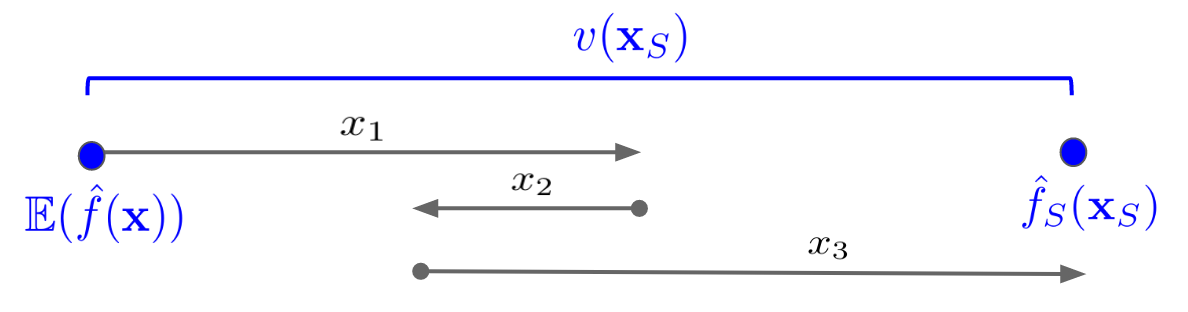
\includegraphics[width=0.5\textwidth, trim=20 0 0 100, clip]{figure_man/shapley_valuefct}}
\resizebox{0.9\linewidth}{!}{
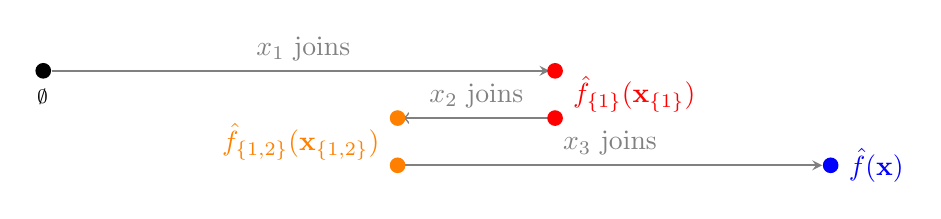
\begin{tikzpicture}[
dot/.style = {circle, fill, inner sep=2pt},
arrow/.style = {-stealth, gray, semithick}
]
% --- main nodes --------------------------------------------------------------
\node[dot, black, label={[black]below:$\fh_\emptyset$}] (start) at (0,0) {};
\node[dot, blue, label={[blue]right:$\hat f(\mathbf x)$}] (end) at (10,-1.2) {};
% --- x1 ----------------------------------------------------------------------
\draw[arrow, shorten >=2pt] (start) -- (6.5,0) node[midway,above] {$x_1$ joins};
\node[dot, red] at (6.5,0) {};
\node[dot, white, label={[red]right:$\hat f_{\{1\}}(\mathbf x_{\{1\}})$}] at (6.5,-.3) {};
% --- x2 ----------------------------------------------------------------------
\coordinate (x2R) at (6.5,-.6);
\coordinate (x2L) at (4.5,-.6);
\draw[arrow, ->, shorten >=2pt] (x2R) -- (x2L) node[midway,above] {$x_2$ joins};
\node[dot, red] at (x2R) {};
\node[dot, orange] at (x2L) {};
% --- x3 ----------------------------------------------------------------------
\coordinate (x3L) at (4.5,-1.2);
\draw[arrow] (x3L) -- (end) node[midway,above] {$x_3$ joins};
\node[dot, orange] at (x3L) {};
\node[dot, white, label={[orange]left:$\hat f_{\{1,2\}}(\mathbf x_{\{1,2\}})$}] at (4.5,-.9) {};
\end{tikzpicture}
}
\end{itemizeS}
\end{framev}
\begin{framev}[align=top]{Shapley Value - Definition \furtherreading{SHAPLEY1953} \furtherreading{STRUMBELJ2014}}
\textbf{Order definition:} Shapley value $\phi_j(\xv)$ quantifies contribution of $x_j$ via
$$
\phi_j(\xv) = \frac{1}{|P|!} \sum_{\tau \in \Pi} \underbrace{\fh_{\Stauj}(\xv_{\Stauj}) - \fh_{\Stau}(\xv_{\Stau})}_{\Delta(j, \Stau)~\text{marginal contribution of feature $j$}}
$$ %S \subseteq P\setminus \{j\}
\begin{itemizeM}
\item \textbf{Interpretation:} $\phi_j(\xv)$ quantifies how much feature $x_j$ contributes to the difference between $\fh(\xv)$ and the mean prediction $\fh_\emptyset$\\
%$x_j$ contributed $\phi_j$ to difference between $\fh(\xv)$ and mean prediction\\
$\leadsto$ Marginal contributions and Shapley values can be negative
\item \textbf{Exact computation of $\phi_j$:} Using PD function
%$\fh_{S}(\xv_S) =  \frac{1}{n} \sum_{i=1}^n \fh_S^{(i)}(\xv_S) = \frac{1}{n} \sum_{i=1}^n \fh(\xv_S, \xv_{-S}^{(i)})$ 
$\fh_S(\xv_S) = \frac{1}{n} \sum_{i=1}^n \fh(\xv_S, \xv_{-S}^{(i)})$
yields
$$
\phi_j(\xv) = \frac{1}{|P|!} \sum_{\tau \in \Pi} \frac{1}{n} \sum_{i = 1}^n
\fh(\xv_{\Stauj}, \xv_{\minusStauj}^{(i)}) - \fh(\xv_{\Stau}, \xv_{-\Stau}^{(i)})
$$
$\leadsto$ $\fh_S$ marginalizes over all features not in $S$ using all obs. $i = 1, \ldots, n$\\
$\leadsto$ Exact computation requires $|P|! \cdot n$ marginal contribution terms
\end{itemizeM}
\spacer[0.25]
%\tiny
%Shapley, Lloyd S. 1953. $"$A Value for N-Person Games.$"$\\
%\vspace{0.2cm}
%Strumbelj, Erik, Igor Kononenko, Erik Strumbelj, and Igor Kononenko. 2014. $"$Explaining prediction models and individual predictions with feature contributions.$"$
\end{framev}


\begin{framev}[align=top]{Estimation: A Practical Problem}
\begin{itemize}[<+->]
\item \textbf{Exact computation is infeasible for many features:}\\
For $|P| = 10$, the number of permutations is $10! \approx 3.6$ million\\
$\leadsto$ Complexity grows factorially with feature count
\item \textbf{Additional challenge: Estimating marginal predictions (PD funcs)}\\
Each permut. $\tau$ defines a coal. $\Stau$ needing its own estimate of $\fh_{\Stau}(\xv_{\Stau})$\\
$\leadsto$ With $|P|!$ permutations and $n$ data points, the number of such estimates grows rapidly, making marginalization costly
\item \textbf{Solution: Sampling-based approximation}\\
Instead of computing $|P|! \cdot n$ terms, we approximate using $M$ random samples of permutations $\tau$ and data points
\item \textbf{Tradeoff: Accuracy vs. Efficiency}\\
Larger $M$ improves Shapley approximation\\
$\leadsto$ Higher cost, but better fidelity to the exact value
\end{itemize}
\end{framev}


\newcommand{\xk}{\mathbf{x}^{(k)}}

\begin{framev}[align=top]{Approximation Algorithm \furtherreading{STRUMBELJ2014}}
Estimate Shapley value $\phi_j$ of observation $\xv$ for feature $j$:
\begin{enumerate}[<+->]
\item[$\bullet$] \textbf{Input:} $\xv$ obs. of interest, $j$ feat. of interest, $\fh$ model, $\D$ data, $M$ iterations
\item For $m = 1, \ldots, M$ \textbf{do}:
\begin{enumerate}
\item Sample random permut. $\tau = (\tau^{(1)}, \ldots, \tau^{(p)}) \in \Pi$ of feature indices% = (\tau^{(1)}, \ldots, \tau^{(p)})
\item Let coalition $\Sm := \Stau$ be the set of features preceding $j$ in $\tau$
\item Sample random data point {\color{blue} $\mathbf{z}^{(m)} \in \D$} (so-called background data)%\\
\item Construct two hybrid obs. by combining values from $\xv$ and {\color{blue} $\mathbf{z}^{(m)}$}:
\begin{itemizeS}
\item $
\xjp = (x_{\tau^{(1)}}, \ldots, x_{\tau^{(|\Sm|)}}, x_j,
{\color{blue}z_{\tau^{(|\Sm|+2)}}^{(m)}, \ldots, z_{\tau^{(p)}}^{(m)}})
$\\
$\leadsto$ includes $\xv_{\Smj}$ (features in $\Sm \cup \{j\}$ from $\xv$), rest from {\color{blue} $\mathbf{z}^{(m)}$}
\item $
\xjm = (x_{\tau^{(1)}}, \ldots, x_{\tau^{(|\Sm|)}},
{\color{blue}z_j^{(m)}, z_{\tau^{(|\Sm|+2)}}^{(m)}, \ldots, z_{\tau^{(p)}}^{(m)}})
$\\
$\leadsto$ includes $\xv_{\Sm}$ (features in $\Sm$ excl. $x_j$ from $\xv$), rest from {\color{blue} $\mathbf{z}^{(m)}$}
\end{itemizeS}
\item Compute marginal contribution $\Delta(j, \Sm) = \fh(\xjp) - \fh(\xjm)$ %\\
\end{enumerate}
\item Compute Shapley value $\phi_j = \frac{1}{M}\sum_{m=1}^M \Delta(j, \Sm)$ %= \frac{1}{M} \sum_{m = 1}^M   \fh(\xjp ) -  \fh(\xjm ) $
\item[$\leadsto$] Over $M$ iterations, the PD functions $\fh_{\Sm}(\xv_{\Sm})$ and $\fh_{\Smj}(\xv_{\Smj})$ are approximated by $\fh(\xjm)$ and $\fh(\xjp)$, where features not in the coalition (to be marginalized) are imputed with vals from random data points {\color{blue} $\mathbf{z}^{(m)}$}
\end{enumerate}
\end{framev}

\begin{framev}[align=top]{Shapley value approx. - Illustration}
\begin{exampleblock}{Definition}
$$
\tikzmark{phi}\phi_{\tikzmark{j}j}(%\tikzmark{v}\fh,
\tikzmark{x}\xv)=\frac{1}{M}\tikzmark{M}\sum_{m=1}^M \left[
\fh(\xv_{+j}\tikzmark{SJ}^{(m)}) -
\fh(\xv_{-j}\tikzmark{S}^{(m)})\right]
$$

\begin{tikzpicture}[
remember picture,
overlay,
expl/.style={draw=blue,fill=white,rounded corners,text width=3.7cm},
arrow/.style={blue,ultra thick,->,>=latex}
]
\node<1>[expl] 
(xex) 
at (4,2cm)
{$\xv$: obs. of interest};
\draw<1>[arrow]
(xex.south) to[out=270,in=90] ([xshift= 0.5ex, yshift=1.5ex]{pic cs:x}); 
\node<1>[expl] 
(Sex) 
at (9,2cm)
{$\xv$ with feature values in $\xv_{\Sm}$ (other are replaced)};
\node<2>[expl] 
(Sex) 
at (5,2cm)
{Contribution of feature $j$ to coalition $\Sm$};
\node<1>[expl] 
(SJex) 
at (8,-0.8cm)
{$\xv$ with feature values in $\xv_{\Smj}$};
\draw<1>[arrow]
(Sex.south) to[out=270,in=50] ([xshift= 1ex, yshift=2.5ex]{pic cs:S});
\draw<2>[arrow]
(Sex.east) to[out=0,in=90] ([xshift= 1ex, yshift=2.5ex]{pic cs:S});
\draw<1>[arrow]
(SJex.north) to[out=90,in=270] ([yshift=-1ex]{pic cs:SJ}); 
\draw<2> [decorate,decoration={brace, amplitude=5pt,mirror,raise=4ex}]  (5.1,1.1) --  (8.35,1.1)
node[midway,yshift=-3.4em]{\scriptsize $:= \Delta(j, \Sm)$};
\draw<2> [draw=white, fill=white, opacity=0.6]
(2.1,0) -- (5.1,0) -- (5.1,1.5) -- (2.1,1.5) --cycle;
%%%% Explain Formula III
\draw<3> [draw=white, fill=white, opacity=0.6]
(1.2,0) -- (3.5,0) -- (3.5, 2) -- (2.2,2) --cycle;
\draw<3> [draw=white, fill=white, opacity=0.6]
(5.0,0) -- (10.0,0) -- (10.0,2) -- (5.0,2) --cycle;
\node<3>[expl] 
(Mex) 
at (8,2cm)
{average the contributions of feature $j$};
\draw<3>[arrow]
(Mex.west) to[out=180,in=50] ([xshift= 0.5ex, yshift=4ex]{pic cs:M}); 
\end{tikzpicture}
\end{exampleblock}
%\vspace{0.5cm}
\begin{itemizeM}
\begin{onlyenv}<1>
\spacer[2.5]
\end{onlyenv}
\begin{onlyenv}<2>
\item $\Delta(j, \Sm) = \fh(\xjp) - \fh(\xjm)$ is marginal contribution of feature $j$ to coalition $\Sm$
\item Here: Feature \textit{year} contributes +700 bike rentals if it joins coalition $\Sm = \{temp, hum\}$ %compared to the expected prediction conditioned on features in coalition $\Sm$ (while other features were taken from a random obs.)
\end{onlyenv}
\begin{onlyenv}<3>
\item Compute marginal contribution of feature $j$ towards the prediction across all randomly drawn feature coalitions $S_1, \ldots, \Sm$
\item Average all $M$ marginal contributions of feature $j$
\item Shapley value $\phi_j$ is the payout of feature $j$, i.e., how much feature \textit{year} contributed to the overall prediction in bicycle counts of a specific obs. $\xv$
\end{onlyenv}
\end{itemizeM}
\vfill
\begin{center}
% Link https://docs.google.com/presentation/d/14FZZ4zk7IBZv6XnQA0wDVfCDhmjzf4np5uVj7KrIxXg/edit#slide=id.p
\includegraphics<1>[page=13, width=1\textwidth]{figure_man/data_shapley}
\includegraphics<2>[page=14, width=1\textwidth]{figure_man/data_shapley}
\includegraphics<3>[page=15, width=1\textwidth]{figure_man/data_shapley}
\end{center}
\end{framev}





\begin{framev}[align=top]{Revisited: Axioms for Fair Attributions}
We adapt the classic Shapley axioms to the setting of model predictions:
\\
\spacer[0.25]
\begin{itemizeM}%[<+->]
%\itemsep1em
\item \textbf{Efficiency}: Sum of Shapley values adds up to the centered prediction:
$$
\textstyle\sum_{j=1}^p \phi_j(\xv) = \fh(\xv) - \E_\xv[\fh(\xv)]
$$
$\leadsto$ All predictive contribution is fully distributed among features
\item \textbf{Symmetry}: Identical contributors receive equal value:
$$
\fh_{\Scupj}(\xv_{\Scupj}) = \fh_{\Scupk}(\xv_{\Scupk}) \ \forall S \subseteq P \setminus \{j,k\}
\Rightarrow \phi_j = \phi_k
$$
$\leadsto$ Interaction effects are shared equitably
\item \textbf{Dummy (Null Player)}: Irrelevant features receive zero attribution:
$$
\fh_{\Scupj}(\xv_{\Scupj}) = \fh_S(\xv_S) \ \forall S \subseteq P \Rightarrow \phi_j = 0
$$
$\leadsto$ Shapley value is zero for unused features (e.g., trees or LASSO)
\item \textbf{Additivity}: Attributions are additive across models:
$$
\phi_j(v_1 + v_2) = \phi_j(v_1) + \phi_j(v_2)
$$
$\leadsto$ Enables combining Shapley values for model ensembles
\end{itemizeM}
\end{framev}



% \begin{frame}{Additional Estimation Trick}


%   The Shapley value can be estimated more efficiently when certain coalitions are always included in the computation, instead of random sampling:
%   \vspace{0.25cm}
%   \begin{itemize}
%   \itemsep1em
%     \item The coalitions with $S = \emptyset$ (i.e., $|S| = 0$) and $S = \{1, \ldots, p\} \setminus j$ have the highest weights in the Shapley value computation $\leadsto$ including them makes Shapley value more stable with fewer samples %Sample weights have to be adapted for the sampled coalitions afterwards.
%     \item Intuition: Adding a feature to the empty coalition gives information about the \textit{pure} first order effect of the feature, which is the effect without any interactions 
%     \item Adding the feature value to the complete set of feature values gives us the information about the total effect of a feature, which is the sum of the main effect and all interaction effects with other features
%     \item For coalition $S = \emptyset$, there are $0! (|P| - 0 - 1)! = 1 \cdot (|P| - 1)! = (p - 1)!$ orders, which is the same for $S = P \setminus \{j\}$: $|P \setminus \{j\}|! (|P| - |P \setminus \{j\}| - 1)! = (p - 1)! (p - (p-1) - 1)! = (p-1)!$
% \end{itemize}
%  \end{frame}

% \begin{frame}{Additional Estimation Trick}
% An example with $p = 5$ features:
% \vspace{0.25cm}
%     \begin{itemize}
%     \itemsep1em
%         \item There are $5! = 120$ orders in total
%         \item In $(5 - 1)! = 24$ orders, we added feature value $x_j$ to the empty set
%         \item In 24 orders, we added the feature value to the otherwise full feature set
%         \item That means with just two sets, we can already get $\frac{48}{120} = 0.4$ of the contributions to the Shapley value
%         \item Similarly, we could proceed with all coalitions of $\{S: |S| = 1\}$ and $\{S: |S| = p - 1\}$
%         \item When some coalitions are added \enquote{manually}, and the rest are sampled, we have to adapt the weights: Let $w$ be the weight of the \enquote{manually} sampled coalitions, $\hat{\phi}_{j,fixed}$ the part of the Shapley value with only the manual contributions and $\hat{\phi}_{j,sample}$ the Shapley value with the sampled coalitions, then the Shapley value is: $w \cdot \hat{\phi}_{j,fixed} + (1 - w) \hat{\phi}_{j,sample}$
%   \end{itemize}
% \end{frame}

% \begin{frame}{Additional Estimation Trick}
%       \begin{center}
%         
\includegraphics[width=0.5\textwidth]{figure/shapley-weights}
%       \end{center}
% \end{frame}

\begin{framev}[align=top]{Bike Sharing Dataset}
\imageC[0.6]{figure/shapley-bike.pdf}%{figure_man/bike-sharing03.png}%

\begin{itemizeM}%[<+->]
\item Shapley decomposition for a single prediction in bike sharing dataset %(observation $i = 200$)
\item Model pred.: $\fh(\xv^{(200)}) = \textbf{4434.86}$ vs. dataset avg.: $\E_\xv[\fh(\xv)] = \textbf{4507.67}$
\item Total feature attribution: $\sum_j \phi_j = \textbf{-72.81}$\\
$\leadsto$ Explain downward shift from mean prediction
\item Temperature (with value $28.5^\circ$C) -- strongest positive contributor: $+400$
\item \texttt{yr = 2011} and \texttt{days\_since\_2011 = 199} strongly reduce prediction\\
$\leadsto$ Model captures lower bike demand in 2011 compared to 2012
\end{itemizeM}
\end{framev}


% \begin{frame}{Versions of the Shapley Value}

%   \begin{itemize}
%   \item KernelSHAP formulates the Shapley value solution as a regression problem using a specific kernel function. The authors show paralles to LIME and Deeplift.
%   \item TreeSHAP is a fast Shapley value computation method for tree-based models such as gradient boosted trees.
%  \end{itemize}
%     \tiny{Lundberg, Scott M., and Su-In Lee. "A Unified Approach to Interpreting Model Predictions." Advances in Neural Information Processing Systems 30 (2017): 4765-4774.}
%     \tiny{Lundberg, Scott M., Gabriel G. Erion, and Su-In Lee. "Consistent individualized feature attribution for tree ensembles." arXiv preprint arXiv:1802.03888 (2018).}
% \end{frame}

\begin{framev}[align=top]{Advantages and Disadvantages}
\textbf{Advantages:}
\begin{itemizeM}%[<+->]
\item \textbf{Strong theoretical foundation} from cooperative game theory
\item \textbf{Fair attribution:} Prediction is additively distributed across features\\
$\leadsto$ Easy to interpret for users
\item \textbf{Contrastive explanations:} Quantify each feature's role in deviating from the average prediction
\end{itemizeM}
\spacer[0.25]
\textbf{Disadvantages:}
\begin{itemizeM}%[<+->]
\item \textbf{Comput. cost:} Exact computation scales factorially with feature count\\
$\leadsto$ Without sampling, all $2^p$ coalitions (or $p!$ permuts) must be evaluated
\item \textbf{Issue with correlated features:} Shapley values may evaluate the model on feature combinations that do not occur in the real data
\end{itemizeM}
\end{framev}


\endlecture
\end{document}
